\documentclass[a4paper, 12pt]{article}
\usepackage{graphicx}

\usepackage{bera}% optional: just to have a nice mono-spaced font
\usepackage{listings}
\usepackage{xcolor}

\colorlet{punct}{red!60!black}
\definecolor{background}{HTML}{EEEEEE}
\definecolor{delim}{RGB}{20,105,176}
\colorlet{numb}{magenta!60!black}

\lstdefinelanguage{json}{
    basicstyle=\normalfont\ttfamily,
    numbers=left,
    numberstyle=\scriptsize,
    stepnumber=1,
    numbersep=8pt,
    showstringspaces=false,
    breaklines=true,
    frame=lines,
    backgroundcolor=\color{background},
    literate=
     *{0}{{{\color{numb}0}}}{1}
      {1}{{{\color{numb}1}}}{1}
      {2}{{{\color{numb}2}}}{1}
      {3}{{{\color{numb}3}}}{1}
      {4}{{{\color{numb}4}}}{1}
      {5}{{{\color{numb}5}}}{1}
      {6}{{{\color{numb}6}}}{1}
      {7}{{{\color{numb}7}}}{1}
      {8}{{{\color{numb}8}}}{1}
      {9}{{{\color{numb}9}}}{1}
      {:}{{{\color{punct}{:}}}}{1}
      {,}{{{\color{punct}{,}}}}{1}
      {\{}{{{\color{delim}{\{}}}}{1}
      {\}}{{{\color{delim}{\}}}}}{1}
      {[}{{{\color{delim}{[}}}}{1}
      {]}{{{\color{delim}{]}}}}{1},
}


\renewcommand{\figurename}{Fig.}

\begin{document}

\section{Definisi}
Tembang Bali merupakan...

\section{Motivasi}
Tembang Bali merupakan...

\section{Arsitektur Tembang Bali}

\subsection{Arsitektur \textit{Server}}
Sistem Tembang Bali terdiri atas 2 komponen utama yaitu, \textit{server} dan \textit{client}.

\begin{figure}[h]
    \centering
    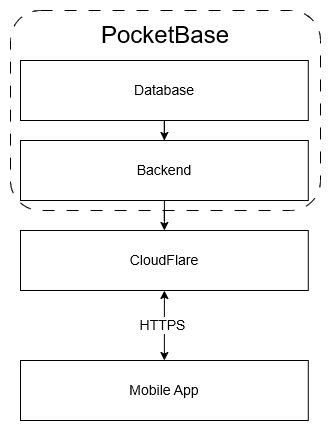
\includegraphics[width=0.5\textwidth]{assets/hla.png}
    \caption{Arsitektur Sistem}
\end{figure}

Client merepresentasikan seluruh aplikasi yang digunakan oleh \textit{end-user} atau pengguna, seperti aplikasi berbasis \textit{Mobile}, \textit{Website}, dsb\
untuk dapat menggunakan layanan yang disediakan oleh \textit{server}.

Server merepresentasikan seluruh komponen aplikasi yang dijalankan pada sisi \textit{server}.\
Hal ini meliputi \textit{Database}, dan \textit{Backend}. Pada sistem ini, seluruh fungsionalitas yang berkaitan dengan \textit{backend} dikelola \
sepenuhnya melalui \textit{framework} bernama PocketBase. PocketBase ini berjalan dalam server, dan dijalankan menggunakan aplikasi berbasis Go.\
Server juga dilindungi oleh Cloudflare, untuk perlindungan eksternal terhadap DDOS, yang juga berfungsi sebagai CDN untuk memperingan kinerja server dalam melayani \textit{request} dari \textit{client}.

\subsection{Arsitektur \textit{Database}}
Pada iterasi awal ini, Tembang Bali menyimpan seluruh data dalam 3 buah tabel, yaitu \textbf{songs}, \textbf{song\_types}, dan \textbf{song\_subtypes}.

\begin{figure}[h]
    \centering
    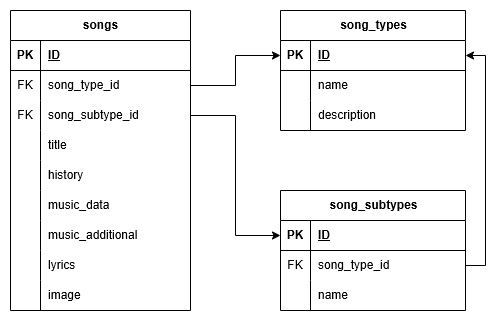
\includegraphics[width=0.8\textwidth]{assets/erd.png}
    \caption{ERD Database}
\end{figure}

\textbf{Tabel songs} terdiri atas \textit{column} \textit{song\_type\_id} dan \textit{song\_subtype\_id} yang berfungsi untuk menyimpan tipe dari data yang disimpan.\
\textit{Column} lainnya berfungsi sebagai \textit{metadata} dan juga lirik.
\textbf{Tabel song\_types} terdiri atas \textit{column} \textit{name} yang berisikan nama tipe dan \textit{description} yang berisi deskripsi singakt mengenai tipe dari data.\
\textbf{Tabel song\_sub\_types} terdiri atas \textit{column} \textit{name} yang berisikan nama tipe dan \textit{song\_type\_id} yang digunakan untuk menandakan relasi dengan \textbf{tabel song\_types}.\

\subsection{Arsitektur \textit{Mobile Client}}

\section{Dokumentasi Public API}
Berikut merupakan dokumentasi \textit{Public API} dari Aplikasi Tembang Bali, yang dapat diakses oleh publik. Untuk saat ini, seluruh sumber daya yang tersedia pada sistem, dapat diakses sepenuhnya oleh masyarakat bebas.\


\section{Dokumentasi PocketBase}
Pada iterasi awal ini, Tembang Bali menyimpan seluruh data dalam 3 buah tabel, yaitu \textit{songs}, \textit{song\_types}, dan \textit{song\_subtypes}.

\subsection*{Song Subtypes}
\textbf{GET} /api/collections/song\_subtypes/records?page=1\&perPage=1

\textbf{search}:

\indent mendapatkan seluruh subtype yang tersedia pada aplikasi

\textit{Response}:
\begin{lstlisting}[language=json,firstnumber=1]
{
    "page": 1,
    "perPage": 30,
    "totalItems": 5,
    "totalPages": 1,
    "items": [
        {
        "collectionId": "wpn5u2qwdejiy6d",
        "collectionName": "song_subtypes",
        "created": "2024-07-03 06:49:40.472Z",
        "id": "wdsyso7rsy259tg",
        "name": "Kidung Dewa Yadnya",
        "song_type": "1uyaj240u3jfxfm",
        "updated": "2024-07-03 06:49:40.472Z"
        }
    ]
}
        \end{lstlisting}

\textbf{view}:

\textbf{GET} /api/collections/song\_subtypes/records/:id

\indent mendapatkan seluruh subtype  yang tersedia pada aplikasi

\textit{Response}:
\begin{lstlisting}[language=json,firstnumber=1]
{
    "id": "RECORD_ID",
    "collectionId": "wpn5u2qwdejiy6d",
    "collectionName": "song_subtypes",
    "created": "2022-01-01 01:00:00.123Z",
    "updated": "2022-01-01 23:59:59.456Z",
    "song_type": "RELATION_RECORD_ID",
    "name": "test"
}
\end{lstlisting}

\subsection*{Song Types}
\textbf{GET} /api/collections/song\_types/records?page=1\&perPage=1

\textbf{search}:

\indent mendapatkan seluruh type yang tersedia pada aplikasi

\textit{Response}:
\begin{lstlisting}[language=json,firstnumber=1]
{
    "page": 1,
    "perPage": 30,
    "totalItems": 5,
    "totalPages": 1,
    "items": [
        {
            "id": "RECORD_ID",
            "collectionId": "3dz70i7dtob7rem",
            "collectionName": "song_types",
            "created": "2022-01-01 01:00:00.123Z",
            "updated": "2022-01-01 23:59:59.456Z",
            "name": "test",
            "description": "test"
        }
    ]
}

\end{lstlisting}

\textbf{view}:

\textbf{GET} /api/collections/song\_types/records/:id

\indent mendapatkan seluruh type yang tersedia pada aplikasi

\textit{Response}:
\begin{lstlisting}[language=json,firstnumber=1]
{
    "id": "RECORD_ID",
    "collectionId": "3dz70i7dtob7rem",
    "collectionName": "song_types",
    "created": "2022-01-01 01:00:00.123Z",
    "updated": "2022-01-01 23:59:59.456Z",
    "name": "test",
    "description": "test"
}
\end{lstlisting}

\subsection*{Songs}
\textbf{GET} /api/collections/song/records?page=1\&perPage=1

\textbf{search}:

\indent mendapatkan seluruh kidung/lagu yang tersedia pada aplikasi

\textit{Response}:
\begin{lstlisting}[language=json,firstnumber=1]
{
    "page": 1,
    "perPage": 30,
    "totalItems": 5,
    "totalPages": 1,
    "items": [
        {
            "id": "RECORD_ID",
            "collectionId": "aqly0n339u404q8",
            "collectionName": "songs",
            "created": "2022-01-01 01:00:00.123Z",
            "updated": "2022-01-01 23:59:59.456Z",
            "song_type": "RELATION_RECORD_ID",
            "song_subtype": "RELATION_RECORD_ID",
            "title": "test",
            "history": "test",
            "music_data": "filename.jpg",
            "music_additonal": "filename.jpg",
            "lyrics": "JSON",
            "lyric_string": "test",
            "image": "filename.jpg"
        }    
    ]
}
\end{lstlisting}

\textbf{view}:

\textbf{GET} /api/collections/song/records/:id

\indent mendapatkan seluruh kidung/lagu yang tersedia pada aplikasi

\textit{Response}:
\begin{lstlisting}[language=json,firstnumber=1]
{
    "id": "RECORD_ID",
    "collectionId": "aqly0n339u404q8",
    "collectionName": "songs",
    "created": "2022-01-01 01:00:00.123Z",
    "updated": "2022-01-01 23:59:59.456Z",
    "song_type": "RELATION_RECORD_ID",
    "song_subtype": "RELATION_RECORD_ID",
    "title": "test",
    "history": "test",
    "music_data": "filename.jpg",
    "music_additonal": "filename.jpg",
    "lyrics": "JSON",
    "lyric_string": "test",
    "image": "filename.jpg"
}
\end{lstlisting}
\end{document}
